In this section we will present the results of the testing that we performed on the project and
present output images from the system that will demonstrate and highlight various effects that
we are able to simulate with the system and compare the results of the system with simalar scenes
created by other systems.

\section{k-d tree performance}
\begin{figure}[h]
\centering
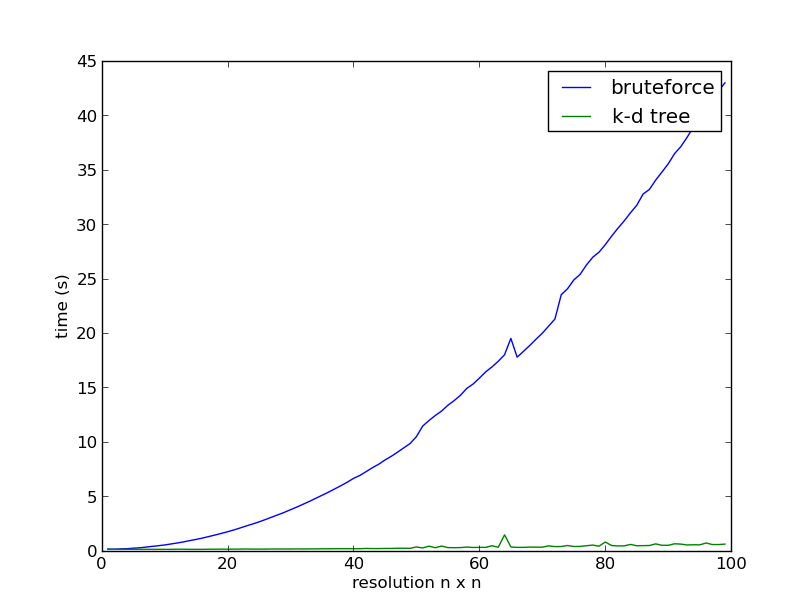
\includegraphics[width=0.7\textwidth]{images/results/tri_intersection.png}
\caption{Comparison of bruteforce and k-d tree mesh intersection test}
\label{fig:bf_kd_comp}
\end{figure}

\section{k-d tree balancing}
\begin{figure}[h]
\centering
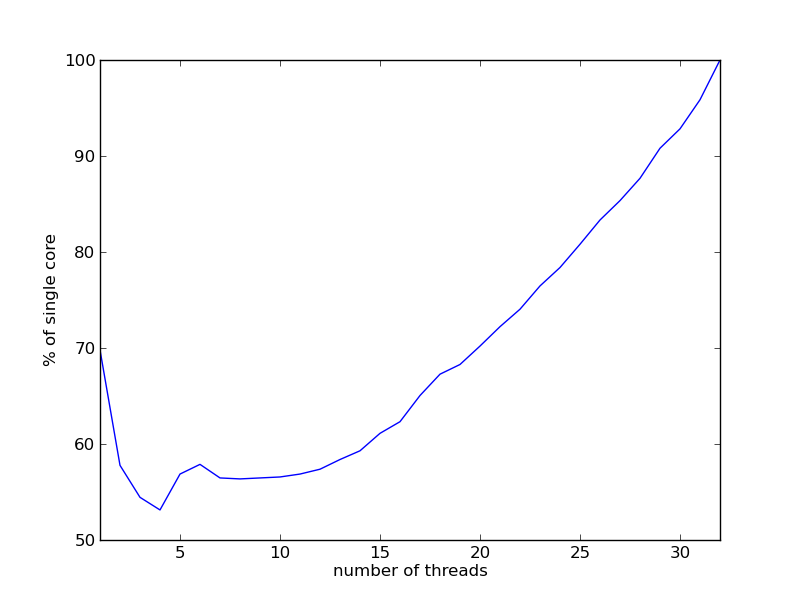
\includegraphics[width=0.7\textwidth]{./images/results/photon_emission_slow_20.png}
\end{figure}

\section{multicore scaling}
\begin{figure}[h]
\centering
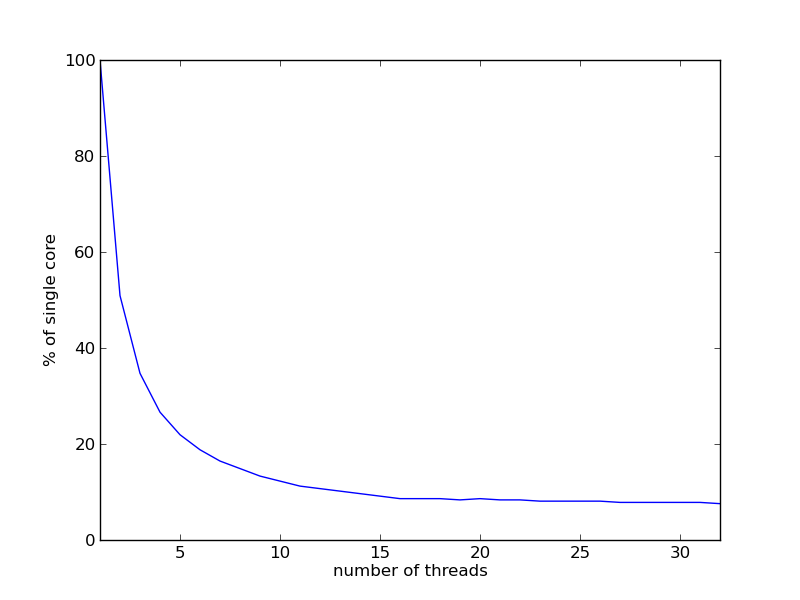
\includegraphics[width=0.7\textwidth]{./images/results/raytrace_multicore.png}
\end{figure}

\section{System Output}

\begin{figure}
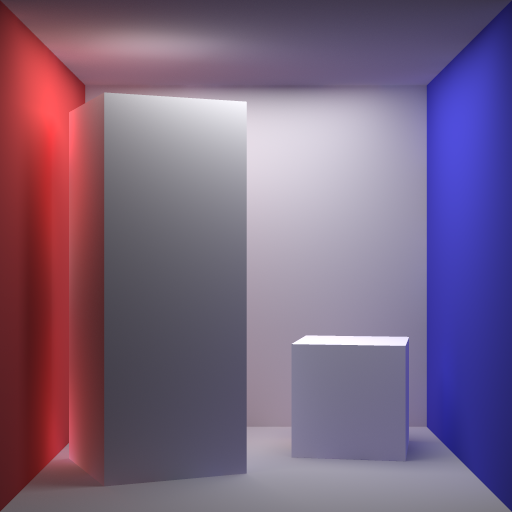
\includegraphics[width=\textwidth]{./images/renders/box.png}
\end{figure}

\begin{figure}
\centering
	\begin{subfigure}[b]{0.6\textwidth}
	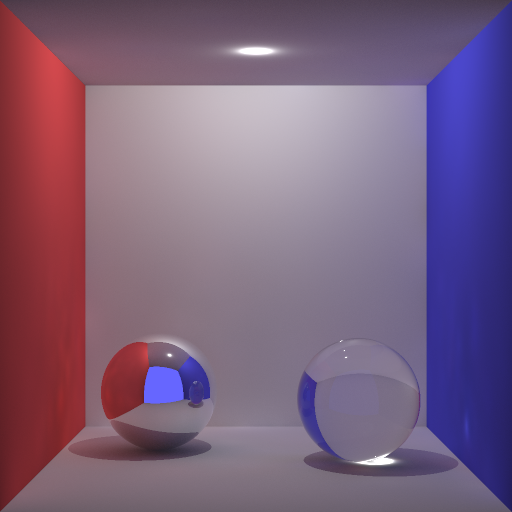
\includegraphics[width=\textwidth]{./images/renders/cornell_box.png}
	\caption{Cornell Box}
	\end{subfigure}

	\begin{subfigure}[b]{0.6\textwidth}
	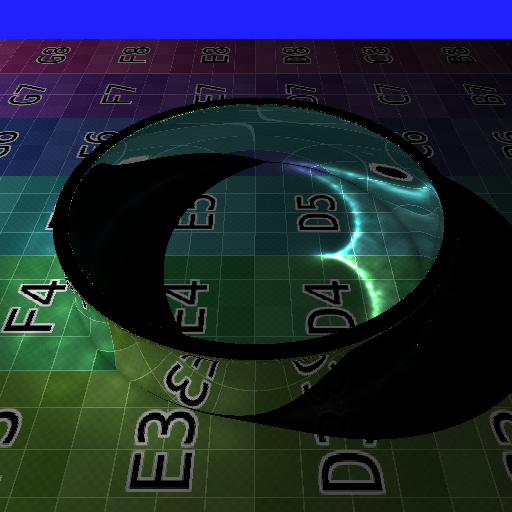
\includegraphics[width=\textwidth]{./images/renders/caustic_ring.png}
	\caption{Caustic Ring}
	\end{subfigure}
\end{figure}

\begin{figure}
\centering
	\begin{subfigure}[b]{0.6\textwidth}
	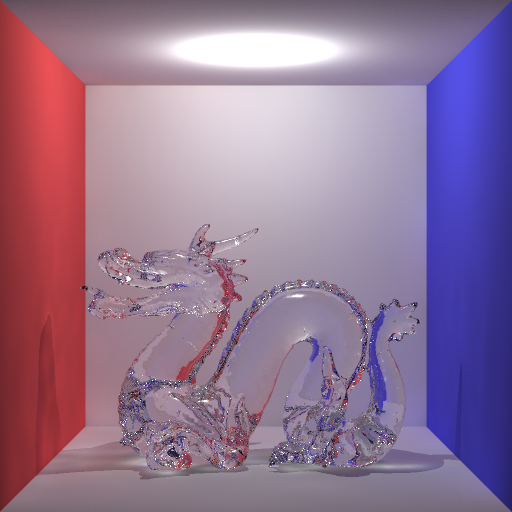
\includegraphics[width=\textwidth]{./images/renders/dragon.png}
	\caption{Stanford Dragon}
	\end{subfigure}

	\begin{subfigure}[b]{0.6\textwidth}
	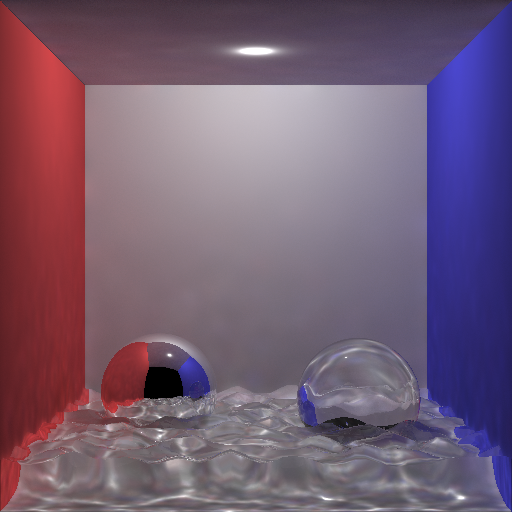
\includegraphics[width=\textwidth]{./images/renders/water.png}
	\caption{Cornell box filled with water}
	\end{subfigure}
\end{figure}

\missingfigure{participating media low}
\missingfigure{participating media high}
